\documentclass[12pt]{article}

\usepackage[utf8]{inputenc}
\usepackage{geometry}
\geometry{a4paper, margin=1in}
\usepackage{graphicx}
\usepackage{hyperref}
\usepackage{fancyhdr}

\setlength{\headheight}{15pt}
\pagestyle{fancy}
\fancyhf{}
\rhead{Computer Workshop Course}
\lhead{Final Assignment}
\rfoot{Page \thepage}

\title{Final project}
\author{abolfazl shahsavari}
\date{January 2024}

\begin{document}

\maketitle
\newpage
\tableofcontents
\newpage

\section{repository link}
\paragraph{\url{https://github.com/abolfazlshahsavary/FinalAssignment}}
\section{Git and GitHub}
\subsection{Repository Initialization and Commits}
\paragraph{Write about how you set up the repository for this assignment. Explain every step in detail?}
\paragraph{To set up a repository, first of all,we must have a GitHub account. After creating a GitHub account or logging into the account, we perform the following steps:}

\begin{itemize}
    \item Go to the repository section in your account
    \item Click on New Repository
    \item Select the repository owner and its name
    \item Enter the explation in the description field
    \item Choose whether your repository is public or private
    \item If you want to add a README to your repository and edit it later
    \item You can add license to tell others the ablity of your code and what they can do with your code
    \item Finally click on create repository 
\end{itemize}
\subsection{GitHub Actions for LaTeX Compilation}
\paragraph{Provide a walkthrough of setting up GitHub Actions to automatically compile your LaTeX
document and any challenges you encountered?}
\paragraph{To launch a compiler for LaTech with Github action, you must set up a workflow and enter your codes for compilation in the main.yml file.\\ Note that you must use tags in this work.
One of the challenges that I faced in this way was the creation of tags, which must first be created from your system and then pushed to the repository.}
\section{Exploration Tasks}
\subsection{Vim Advanced Features}
\paragraph{Explore and document 3 advanced features of Vim that were not covered in class?}
\paragraph{hear of three advance feature in vim:}

\begin{enumerate}
    \item One of Vim's features is macros, with the help of which you can record a sequence of keystrokes that can be executed with only one keystroke. The reason for using this feature is clear from the fact that in text editing and in programming, some tasks need to be executed over and over again. We can call this task repetitive tasks, for example, we can refer to formatting code or generating boilerplate text.
    \item Vim's another feature is a tabbed interface which allows you to open many files and switch between them easily .this can be usefull to save your time while you working. Tabs support multiple windows, making it easy to work with multiple files in same time.
    \item last feature is the folding, which is provided for programmers and some people who work with huge documents, this feature allows you to fold and unfold sections of text, making it easy to navigate and work with large files.this feature is useful for saving time and no need to spend time to transport in large documents.
\end{enumerate}
\subsection{Memory profiling}
\subsubsection{Memory Leak}
\paragraph{In short, explain what memory leaks are and how they might happen in your program?}
\paragraph{A memory leak occurs when a programmer allocates memory and does not free it}
\paragraph{If we don't free the allocated memory, the possibility of memory leak is high}


\subsubsection{Memory profilers}
\paragraph{Read about a tool called Valgrind and write about their purpose and how it helps when memory leaks happen.?}
\paragraph{valgrind is amazing tool witch is use for identification allocated memory.if we allocate a part of memory and we did not free it in purpose and then we open this application we will see that it has tell us about the allocated memory and free memory and the size of memory witch is allocated}
\section{GNU Linux Bash Scripting}
\subsection{fzf}
\paragraph{What is fuzzy searching? Give a short description}
\paragraph{Fuzzy search is one of the search algorithms that, unlike traditional algorithms, allows the user to ignore minor errors such as misspellings or mistakes in one or a few letters of a word.}
\paragraph{Install fzf on your machine and give a description of what the following command does: \texttt{ls | fzf}}
\paragraph{This command makes it easier to navigate and select files and directories, the ls command is used to list all the files and directories in a directory, and with fzf you can do a fuzzy search through your file and the directory is listed.}
\subsection{Using fzf to find your favorite PDF}
\paragraph{You might have came across moments when you want to open up a certain PDF when studying for your final exams but finding the directory of that PDF is a very gruesome and tiring process. In this section, we will be using fzf to find our PDF in seconds! We will be going step by step on how to find your file and use fzf to select it?}
\paragraph{first of all we have to install fd then we can use this command to list all pdf file in that repository \texttt{fd -e pdf} but there is problem here this command list all the pdf file in that repository the better command is \texttt{fd -t -e pdf} that can list all pdf file from that repository and any subrepository }
\paragraph{after listing the pdf file we know the name of pdf that we want to select and we use this command to select it \texttt{fd -t pdf -E '.*' file name | fzf} in this commands \texttt{-t} is for  recursively search texttt{-E '.*'} is use to refer pdf file and fzf select it}

\subsection{Opening the file using Zathura}
\paragraph{to open selected file usinf zathura we can use this command \texttt{fd -t pdf -E '.*' | fzf \&\& zathura (\$cat-)}  I explane any part of commands above instead of \texttt{cat-} this command is used to pass stdin to zathura to open and load your selected file}
\section{Git and FOSS}
\subsection{README.md}
\paragraph{One of the new things that I have come to know is github action git hub action is able to do some commands automatically this repository can compile your latex file to pdf by using of github action in this repository we use tags to identify the latex file . To work with this repository, you just need to add your latex file and create a special tag for your changes and push it to the repository if you want to use this repository follow these steps:}
\begin{enumerate}
    \item fork the repository 
    \item clone it on your machine 
    \item add your latex file to the repository
    \item change the main.yml file to be able to compile your latex file (chnage some thing that are realate to your latex file not the operation) 
    \item create tag for any change in your latex file 
    \item push the tags 
    \item after workflowing your latex file will be released in release section 
    \item 8.after any change following above steps from number 5

\end{enumerate}
subsection{Issues}
\begin{figure}[b]
    \centerline{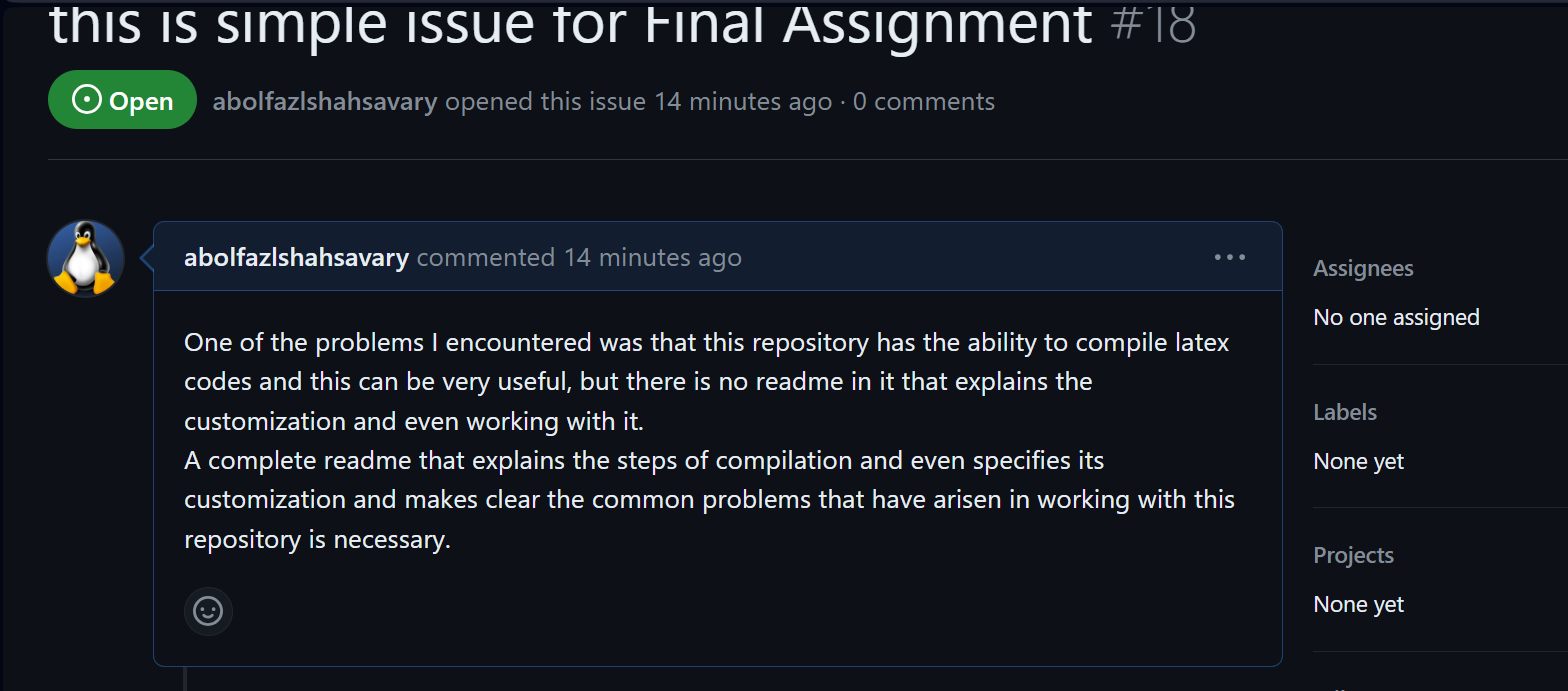
\includegraphics[width=4in, height=2in]{issue.png}}
    \caption{This is my issue.}
    \label{fig}
\end{figure}













\end{document}